\documentclass[UTF8]{ctexart}
%\documentclass[twocolumn]{article}

\usepackage{indentfirst}
\usepackage{caption}
\usepackage{graphicx}
\usepackage{listings}
\usepackage{xcolor}


\lstset{language=C}
\lstset{language=Python}
\lstset{breaklines}
\lstset{extendedchars=false}
\lstset{numbers=left,
frame = single,
title = \lstname} 

\usepackage{algorithm}
\usepackage{algorithmic}
\usepackage{float}

\usepackage{geometry}
\geometry{left = 2.5cm,right = 2.5cm}


\renewcommand{\baselinestretch}{1.5}

\setlength{\parindent}{2em}


\title{操作系统报告}
\author{漆耘含\\2016011058}
\date{}

\begin{document}
\maketitle
\section{快速排序问题}
\subsection{问题综述}
\subsubsection{问题描述}
对于有1,000,000个乱序数据的数据文件执行快速排序。\par
\subsubsection{实验步骤}
(1)首先产生包含1,000,000个随机数(数据类型可选整型或者浮点型)的数据文件;\par
(2)每次数据分割后产生两个新的进程(或线程)处理分割后的数据,每个进程(线程)处理的数据小于1000以后不再分割(控制产生的进程在20个左右);\par
(3)线程(或进程)之间的通信可以选择下述机制之一进行:\par
\qquad 管道(无名管道或命名管道)\par
\qquad 消息队列\par
\qquad 共享内存\par
(4)通过适当的函数调用创建上述IPC对象,通过调用适当的函数调用实现数据的读出与写入;\par
(5)需要考虑线程(或进程)间的同步;\par
(6)线程(或进程)运行结束,通过适当的系统调用结束线程(或进程)。\par
\subsection{实验环境}
Ubuntu\quad 18.04.1 \quad LTS, 64位操作系统\par
具体配置如下:\par
\begin{figure}[!h]
\centering
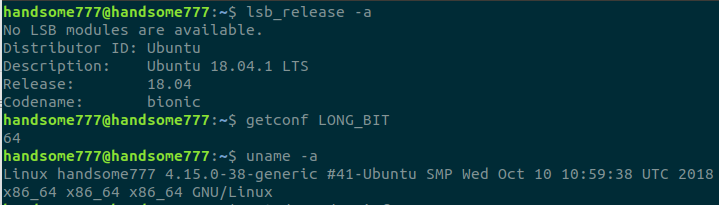
\includegraphics[scale = 0.7,bb=0 0 518 148]{ubuntu_info.png}
\label{img1}
\end{figure}
\subsection{原理分析及实现}
进行进程间通信有三种方法:管道、消息队列、共享内存、我选择的是共享内存的方法。\par
在我设计的方法中,一共有两个主要的对象:管理者(scheduler)和工作者(worker)。管理者负责分发任务,在这个问题中,管理者从队列中取出排在最前面的一个序列,然后将其分配给一个工作者,工作者得到这个序列之后,如果序列长度小于等于1000,则直接调用系统快排函数进行排序;如果序列长度大于1000,则根据快速排序算法将其分为两个块,然后将着两个块放入队列的末尾。下面将对这两个对象进行详细的描述。\par
\subsubsection{管理者(scheduler)}
管理者进程在创建之后,会不停地检查队列是否为空,如果队列为空,同时正在工作的工作者数量为0,则说明排序结束,程序结束;如果队列为空,但正在工作的工作者数量不为0,说明排序还未结束,因此应陷入等待状态,直到一个工作者结束工作,将其唤醒,当工作者全部结束工作,则处于前面描述的情况,排序结束,退出程序。\par
当队列不为0,说明排序还在进行中,当目前工作者数量小于最大工作者数量的时候,从队列中读取最前面的一个序列,然后创建一个新工作者进程,让其对该序列进行操作(调用排序算法或者将其分为两个块并放入队列);如果当前工作者数量达到最大,则需要等待某一工作者结束任务(释放进程),管理者再进行分配任务。\par
需要注意的是,在操作队列的时候,一定要先锁住再进行操作,防止多个进程同时对队列进行操作,引起混乱。\par
管理者程序流程如下:\par
\begin{algorithm}
\caption{scheduler algorithm}
\begin{algorithmic}[1]
\STATE while(1)\par
\STATE	\qquad 锁住scheduler,防止对个进程操作队列;\par
\STATE	\qquad if(队列为空)	\par
\STATE	\qquad\qquad if(工作者数量==0)	\par
\STATE	\qquad\qquad\qquad break;	\par
\STATE \qquad \qquad else \par
\STATE	\qquad\qquad\qquad 等待直到一个工作者结束进程将其唤醒;\par
\STATE	\qquad\qquad \qquad 解锁scheduler;\par
\STATE	\qquad else if(当工作者的数量 < 工作者最大数量)\par
\STATE	\qquad\qquad 创建一个新worker进程;\par
\STATE	\qquad\qquad 解锁scheduler;\par 
\STATE	\qquad else \qquad //因为此时工作者数量达到饱和\par
\STATE	\qquad\qquad 等待一个工作者结束进程将其唤醒;\par
\STATE	\qquad \qquad 将scheduler解锁\par
\end{algorithmic}
\end{algorithm}

\subsubsection{工作者(worker)}
工作者在得到管理者分配的任务之后,先判断得到序列的长度(L)是否小于等于1000,如果L小于等于1000,则直接调用qsort进行排序;如果L大于1000,则需要对这个序列进行划分,设立两个变量分别指向序列的最左端和最右端的元素,并设置一个中间元素pivot,从左往右找第一个大于pivot的元素,标记为k,如果整个序列都没找到,则说明已经排好序了;同时从右往左找第一个小于pivot的元素,标记为h,如果整个序列都没找到,则序列已经是有序的;当k $\geq $ h的时候,说明该序列已经可以分为左右两个子序列,左序列的任意值都小于右序列,因此将这两个子序列放入队列;如果k $\leq $h,则交换k和h,继续上述算法,直到该序列可以分为左右两个子序列,左边序列的每一个值都小于右边序列的值。\par
在完成序列划分或排序任务之后,该工作者的任务已经完成,这时发出一个信号唤醒正处于阻塞的cond,然后删除该工作者进程。\par
\begin{algorithm}
\caption{worker algorithm}
\begin{algorithmic}[1]
\STATE if(序列长度小于等于1000)\par
\STATE	\qquad 调用函数进行排序;\par
\STATE	else	\par
\STATE	\qquad 	while(1)\par
\STATE	\qquad\qquad 从左往右找第一个大于pivot的元素(k)\par
\STATE	\qquad\qquad \qquad 如果整个序列都没有,break;\par
\STATE \qquad \qquad 从右往左找第一个小于pivot的元素(h)\par
\STATE	\qquad\qquad\qquad 如果整个序列都没有,break;\par
\STATE	\qquad\qquad if(k $\geq$ h)\par
\STATE	\qquad\qquad \qquad break;\par
\STATE	\qquad \qquad 交换k和h对应的元素;\par
\STATE	\qquad 将左右两个序列放入队列;\par
\STATE	工作者完成任务,数量-1;\par 
\STATE	唤醒正处于阻塞的cond并结束进程;\par
\end{algorithmic}
\end{algorithm}
\par

\subsubsection{程序总流程}
在程序刚开始的时候,先生成一百万个浮点数,然后初始化mutex变量和cond变量,创建管理者进程(scheduler),等待整个进程结束,检查元素是都已经有序(即检查快速排序是否正确)。\par
主函数流程如下所示:\par
\begin{algorithm}
\caption{main function}
\begin{algorithmic}[1]
\STATE 生成一百万个随机浮点数;\par
\STATE 初始化mutex和cond变量;\par
\STATE 将整个序列放入队列中;\par
\STATE 创建管理者(scheduler)进程;\par
\STATE \qquad 不断创建工作者进程进行排序或序列划分;\par
\STATE 等待管理者进程结束;\par
\STATE 检查快速排序结果是否正确;\par
\STATE 程序结束;\par
\end{algorithmic}
\end{algorithm}

\subsection{结果展示及分析}
\subsubsection{生成的随机浮点数序列}
\begin{figure}[!h]
\centering
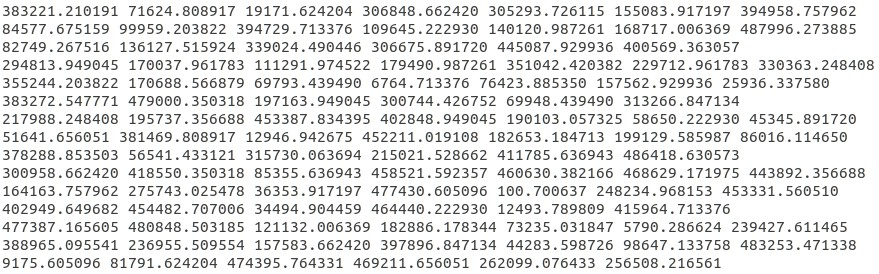
\includegraphics[scale = 0.7,bb=0 0 633 197]{2_random.jpg}
\label{img2}
\end{figure}

\subsubsection{运行过程}
设置的工作者最大数量为20,因此当有20个工作者的时候,需要等待,如下图所示:\qquad \par
\begin{figure}[!h]
\centering
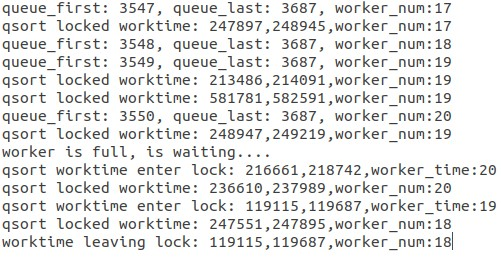
\includegraphics[scale = 0.7,bb=0 0 361 186]{2_workerfull.jpg}
\label{img4}
\end{figure}
当队列为空但线程还没运行结束的时候:\par
\begin{figure}[!h]
\centering
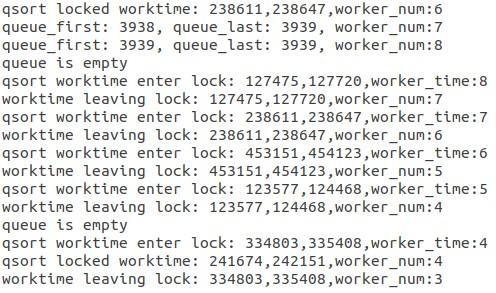
\includegraphics[scale = 0.7,bb=0 0 357 211]{2_queue_empty.jpg}
\label{img5}
\end{figure}
在排序结束之后,判断快速排序是否正确:\par
\begin{figure}[!h]
\centering
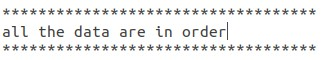
\includegraphics[scale = 0.7,bb=0 0 234 43]{2_check.jpg}
\label{img6}
\end{figure}

\subsection{性能分析}
通过设置不同的工作者最大数量,根据快速排序的运行时间来研究算法性能:\par
\par
\begin{tabular}{|c|c|c|c|c|c|c|c|c|c|}
\par
\hline
工作者最大数量&2&5&10&15&20&25&30&35&100\\
\hline
运行时间(ms)&344&210&200&195&193&196&197&183&182\\
\hline
\end{tabular}
\qquad \par
由上述表格可以看出,当在最大工作者数量比较小的时候,性能随着工作者数量的增大而变好,但当最大工作者数量比较大的时候,性能没有明显的提高,原因是因为CPU的运算速度比较快,排序一百万个数据最多可能会用到35-45个工作者,因此当最大工作者一直增大的时候,用到的工作者并没有增多,因此性能不会明显提升。\par

\subsection{思考题}
\subsubsection{你采用了你选择的机制,而不是另外两种机制解决该问题,请解释你做出这种选择的理由}
本次实验是使用的内存共享的方法。\par
因为快速排序本来就是一个CPU密集型的任务,在不进行IO的时候速度是比较快的,如果采用管道来进行多进程间待排序和排序序列的传递,是很没有效率的,性能不太好;用消息队列传递任务,并用共享内存来实现数据共享,则和我上述的算法类似,不过进程间的开关和内存映射开销比线程要高。\par
因此我使用多线程+共享内存的方法。\par

\subsubsection{你认为另外两种机制是否可以解决该问题,如果可以,请给出你的思路,如果不能,请解释理由}
另外两种方法都是可以的。\par
管道:创建主进程与多个工作者进程,主进程通过管道将待排序序列传给工作者,工作者将排序完成的结果和新任务传递给主进程,主进程在内存中不断更新数据段。\par
消息队列:任务由消息队列在主进程和工作者之间来回传递,主进程直接将任务放入消息队列即可,进程间纯粹使用共享内存,与本实验方法类似。\par

\subsection{运行代码指令}
1. gcc -o main main.c -lpthread\par
2. ./main

\subsection{第二次实验总结}
因为之前进行过第一次实验,对多线程编程有了初步的了解和认识,因此第二次实验上手特别快,比较顺利地完成,在完成编程任务之后,还通过设置不同的工作者最大数量,来对算法的性能进行剖析,让我对多线程快速排序算法的性能有更深的认识。同时,本次试验还帮助我复习了快速排序算法,收货很多!



\section{管道驱动程序开发}
\subsection{问题描述}
管道是现代操作系统中重要的进程间通信(IPC)机制之一,Linux和Windows操作系统都支持管道。\par
管道在本质上就是在进程之间以字节流方式传送信息的通信通道,每个管道具有两个端,一端用于输入,一端用于输出,如下图所示。在相互通信的两个进程中,一个进程将信息送入管道的输入端,另一个进程就可以从管道的输出端读取该信息。显然,管道独立于用户进程,所以只能在内核态下实现。\par

\begin{figure}[!h]
\centering
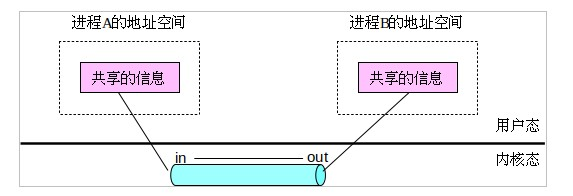
\includegraphics[scale = 0.7,bb=0 0 413 141]{5_1.jpg}
\label{img7}
\end{figure}

在本实验中,请通过编写设备驱动程序mypipe实现自己的管道,并通过该管道实现进程间通信。\par
你需要编写一个设备驱动程序mypipe实现管道,该驱动程序创建两个设备实例,一个针对管道的输入端,另一个针对管道的输出端。另外,你还需要编写两个测试程序,一个程序向管道的输入端写入数据,另一个程序从管道的输出端读出数据,从而实现两个进程间通过你自己实现的管道进行数据通信。\par
\subsection{原理分析及实现}
\subsubsection{模块框架}
本次试验创建的是字符设备驱动程序,并且实验环境是在linux下,因此需要用GPL协议,这样才能正确的和内部函数进行对接。同时,在linux下要装载驱动程序和卸载的时候,需要使用insmod和rmmod来进行,因此需要用相应的宏来指定这两个函数。具体如下:\par

\lstset{language = c}
\begin{lstlisting}
/***********module*******************/
MODULE_LICENSE("GPL");
MODULE_AUTHOR("handsome777");

module_init(driver7_init);
module_exit(driver7_exit);

\end{lstlisting}

Linux通过$file\_operations$结构访问驱动程序的函数,这个结构的每一个成员都对应着一个调用,用户进程利用对设备文件进行read/write操作的时候,系统调用通过设备文件的主设备号找到相应的设备驱动程序,然后读取这个数据结构相应的函数指针,接着吧控制权交给该函数,这就是Linux的设备驱动程序工作的基本原理,本次使用用到的结构体如下所示:\par
\lstset{language = c}
\begin{lstlisting}
struct file_operations driver7_ops = 
{
    .owner = THIS_MODULE,
    .open  = driver7_open,
    .read  = driver7_read,
    .write = driver7_write,
    .release = driver7_release
};
\end{lstlisting}
\par
其中,第一个成员owner不是一个操作,而是一个指向拥有这个结构的模块的指针,$THIS\_MODULE$是在$<linux/module.h>$中定义的宏,一般初始化为$THIS\_MODULE$。\par
第二个成员是open,这是对设备文件进行的第一个操作,如果这一个项是NULL,则设备打开是成功的,但驱动是不会得到通知的,其函数要求以及本程序实现如下:\par
\lstset{language = c}
\begin{lstlisting}
int (*open) (struct inode * inode , struct file * filp );
int driver7_open(struct inode * inode, struct file *filp);
\end{lstlisting}
\par
与open操作对应的是release操作,当最后一个打开设备的用户执行close()系统调用的时候,内核将调用驱动程序release()函数,主要任务是清理未结束的输入输出操作,释放资源等,其函数要求以及本程序实现如下:\par
\lstset{language = c}
\begin{lstlisting}
int (*release) (struct inode *, struct file *);
int driver7_release(struct inode *inode, struct file *filp);
\end{lstlisting}

接下来是read操作,该函数是用来从设备中获取数据,在这个位置的一个空指针导致read系统调用以-EINVAL("Invalid argument")失败。一个非负返回值代表了成功读取的字节数(返回值是一个“signed size”类型),具体的函数要求以及本程序实现如下:\par
\lstset{language = c}
\begin{lstlisting}
ssize_t (*read) (struct file * filp, char __user * buffer, size_t    size , loff_t * p);
ssize_t driver7_read(struct file *filp, char __user *buf, size_t count, loff_t *f_pos);
\end{lstlisting}

其中的指针参数filp为进行读取信息的目标文件,指针参数buffer为对应防止信息的缓冲区(即用户空间内存地址),参数size为要读取的信息长度,参数p为读的位置相对于文件开头的偏移,在读取信息后,这个指针一般都会移动,移动的值为要读取信息的长度值。\par

最后是write操作,即发送数据给设备,如果NULL,则返回-EINVAL给调用write操作的程序,如果非负,返回值代表成功写的字节数。具体的函数要求以及本程序实现如下:\par
\lstset{language = c}
\begin{lstlisting}
ssize_t(*write)(struct file *filp,const char __user *buffer,size_t count,loff_t *ppos);
ssize_t driver7_write(struct file *filp, const char __user *buf, size_t count, loff_t *f_pos);
\end{lstlisting}

\subsubsection{初始化函数}
在初始化模块的时候,需要创建struct class,分配设备号,为每个设备文件分配缓存区,初始化$driver\_dev$结构体,并且为每个设备文件设置cdev结构体并注册,映射新建设备文件。\par
其中,$driver7\_dev$是自己定的,具体的如下:\par
\lstset{language = c}
\begin{lstlisting}
//devices struct
struct driver7_dev
{
	struct semaphore sem;
	struct cdev cdev;
	void* data;
	int begin_position;
	int end_position;
	int curr_size;
	int size;
	wait_queue_head_t in_queue;
	wait_queue_head_t out_queue;
};
\end{lstlisting}
里面的元素有每个设备文件进行读写的结构体、缓存区、缓存区大小、当前大小、头尾指针、以及阻塞需要使用的$wait\_queue\_head\_t$,读和写都需要,以及读写互斥信号量sem、同时还需要一个cdev。\par
cdev是内核中注册字符设备的结构体,通过cdev可以决定本字符设备驱动行为的IO函数,因此需要把结构体指针struct file$\_$operations* 赋给cdev中相应的环境变量。\par
具体的实现流程如下:\newpage
\begin{algorithm}
\caption{driver7$\_$init}
\begin{algorithmic}[1]
\STATE 创建class(class$\_$create);\par
\STATE 修改新建设备文件的权限;\par
\STATE 分配设备号;\par
\STATE 得到主设备号(MAJOR);\par
\STATE 分配缓存区数组空间(kmalloc);\par
\STATE 将driver$\_$dev中结构体清零(memset);\par
\STATE 对每一个设备;\par
\STATE \qquad 分配缓冲区、设置缓存区大小、头尾指针以及当前使用大小;\par
\STATE \qquad 初始化信号量、等待队列头;\par
\STATE \qquad 设置并注册cdev结构体(driver$\_$setup$\_$cdev);\par
\end{algorithmic}
\end{algorithm}
其中,driver7$\_$init函数调用了driver$\_$setup$\_$cdev函数来进行设置并注册cdev结构体,其具体流程如下:\par
\begin{algorithm}
\caption{driver7$\_$setup$\_$cdev}
\begin{algorithmic}[1]
\STATE 在内核中初始化字符设备驱动的cdev结构体(cdev$\_$init);\par
\STATE 设置cdev的owner;\par
\STATE 设置字符驱动的file$\_$operations为实现的IO操作函数;\par
\STATE 在内核中注册cdev(cdev$\_$add);\par
\STATE 创建设备文件(device$\_$create);\par
\STATE 将driver$\_$dev中结构体清零;\par
\STATE 对每一个设备;\par
\STATE \qquad 分配缓冲区、设置缓存区大小、头尾指针以及当前使用大小;\par
\STATE \qquad 初始化信号量、等待队列头;\par
\STATE \qquad 设置并注册cdev结构体;\par
\end{algorithmic}
\end{algorithm}

\subsubsection{卸载函数}
卸载顺序和初始化顺序相反,删除设备文件、注销cdev、释放缓存区、注销struct class、注销设备号分配,具体实现流程如下:\par
\begin{algorithm}
\caption{driver7$\_$exit}
\begin{algorithmic}[1]
\STATE 对每一个设备;\par
\STATE \qquad 删除设备文件(device$\_$destroy);\par
\STATE \qquad 注销对应的cdev(cdev$\_$del);\par
\STATE \qquad 释放缓存区(kfree);\par
\STATE 注销class(class$\_$destroy);\par
\STATE 注销设备号(unregister$\_$chrdev$\_$region);\par
\STATE 释放缓存区指针数组(kfree);\par
\end{algorithmic}
\end{algorithm}

\subsubsection{IO函数}
读写函数本质上是一个循环列表读写数据,但比较关键的是要互斥,即对同一个设备,只能一个读或者写,不能同时进行操作,因此使用信号量实现。同时当写操作的时候,如果缓存区已经写满,这时应该进行阻塞;如果是读操作,如果缓存区已经为空,则也应该进行阻塞。\par
下面展示写操作函数流程:\par
\begin{algorithm}
\caption{driver7$\_$write}
\begin{algorithmic}[1]
\STATE 从filp中获得driver7$\_$dev的结构体指针;\par
\STATE 申请信号量;\par
\STATE 如果缓存区满,则等待直到读操作读取一部分内容;\par
\STATE 确保只写到缓存区满;\par
\STATE 如果数据分布在数组两端;\par
\STATE \qquad 更新当前大小、已经完成的大小、尾指针;\par
\STATE 从用户空间读取数据;\par
\STATE 更新当前缓存区中存储数据大小、尾部指针;\par
\STATE 释放信号量;\par
\STATE 唤醒阻塞的读操作,如果有的话;\par
\end{algorithmic}
\end{algorithm}

读操作也是类似的,下面展示读操作函数流程:\par
\begin{algorithm}
\caption{driver7$\_$read}
\begin{algorithmic}[1]
\STATE 从filp中获得driver7$\_$dev的结构体指针;\par
\STATE 申请信号量;\par
\STATE 如果缓存区为空,则等待直到写操作写入一点东西;\par
\STATE 如果数据分布在数组两端;\par
\STATE \qquad 更新当前大小、已经完成的大小、尾指针;\par
\STATE 向用户控件写入数据;\par
\STATE 更新当前缓存区中存储数据大小、尾部指针;\par
\STATE 释放信号量;\par
\STATE 唤醒阻塞的写操作,如果有的话;\par
\end{algorithmic}
\end{algorithm}


\subsubsection{编译模块}
编译模块是通过编写make文件来进行的,具体代码如下:\par
\lstset{language = make}
\begin{lstlisting}
obj-m :=driver7.o
KDIR  := /lib/modules/$(shell uname -r)/build
PWD   := $(shell pwd)
default:
	$(MAKE) -C $(KDIR) M=$(PWD) modules
\end{lstlisting}
KDIR是当前运行内核同版本的源码目录。

以上模块的具体的代码见附件。

\subsection{测试结果}
\subsubsection{加载和卸载}
通过make进行编译之后生成driver7.ko文件,通过在终端输入insmod driver7.ko装载,结果如下:\par
在字符设备列表中结果(/proc/devices):\newpage
\begin{figure}[!h]
\centering
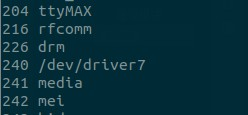
\includegraphics[scale = 1.0,bb=0 0 179 83]{5_2.jpg}
\label{img7}
\end{figure}
通过在终端输入ls -l /dev,可以看到:\par
\begin{figure}[!h]
\centering
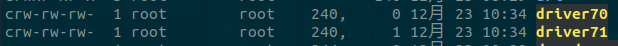
\includegraphics[scale = 1.0,bb=0 0 445 33]{5_3.png}
\label{img8}
\end{figure}
在/var/log/kern.log中,可以看到加载的信息:\par
\begin{figure}[!h]
\centering
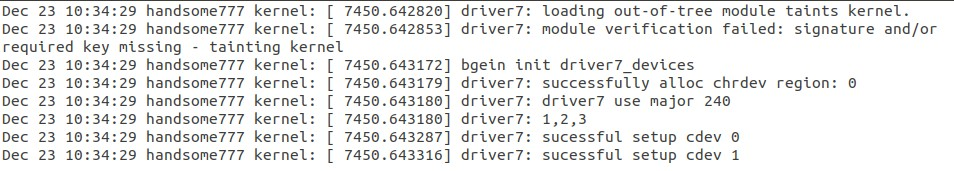
\includegraphics[scale = 0.6,bb=0 0 687 123]{5_4.jpg}
\label{img9}
\end{figure}
通过在终端输入lsmod可以看到加载的信息:\par
\begin{figure}[!h]
\centering
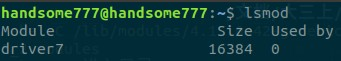
\includegraphics[scale = 1.0,bb=0 0 246 44]{5_5.jpg}
\label{img10}
\end{figure}

由此可见,加载成功。如果要卸载,则在终端输入rmmod driver7即可。在kern.log中可以看到:\par
\begin{figure}[!h]
\centering
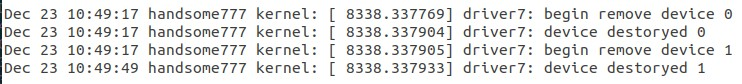
\includegraphics[scale = 0.7,bb=0 0 534 60]{5_6.jpg}
\label{img10}
\end{figure}
上图表明卸载成功。

\subsubsection{验证读写操作}
读写操作通过编写两个.c程序来验证,写操作是每隔一段时间就向缓冲区里面进行写操作,读操作同样也是,如果先进行写操作而不进行读操作,则写入一段时间之后,则会陷入阻塞,因为这个时候缓冲区已经满了,除非进行读操作才会继续写操作。\par
下面是写操作时的运行结果和kern.log中的结果:\par
\begin{figure}[!h]
\centering
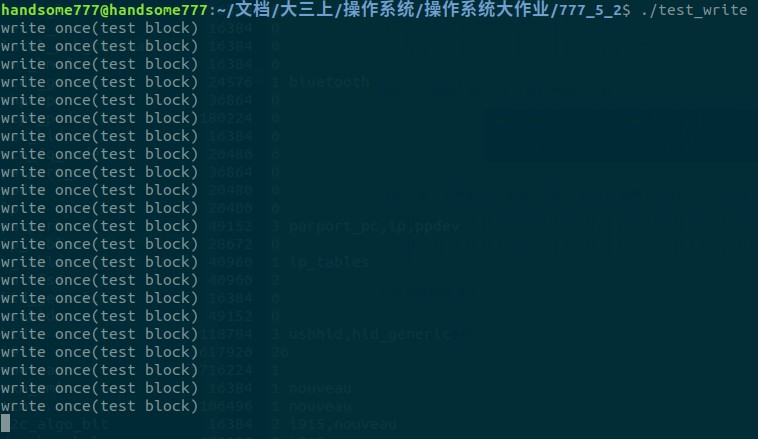
\includegraphics[scale = 0.7,bb=0 0 546 316]{5_7.jpg}
\label{img10}
\end{figure}
kern.log\par
\begin{figure}[!h]
\centering
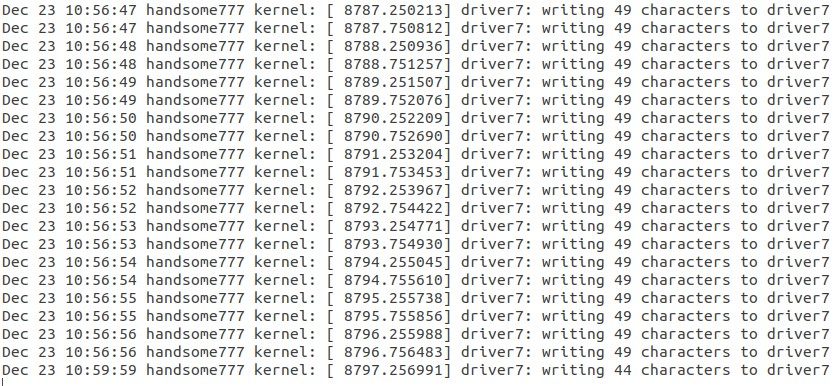
\includegraphics[scale = 0.7,bb=0 0 603 278]{5_8.jpg}
\label{img11}
\end{figure}

然后运行read程序,这时可以看到第一次会读出缓存区中的所有数据,然后write程序开始继续写,read也相应地在读取,这时,将write程序关掉,读操作应该会陷入阻塞,具体如下:\newpage
\begin{figure}[!h]
\centering
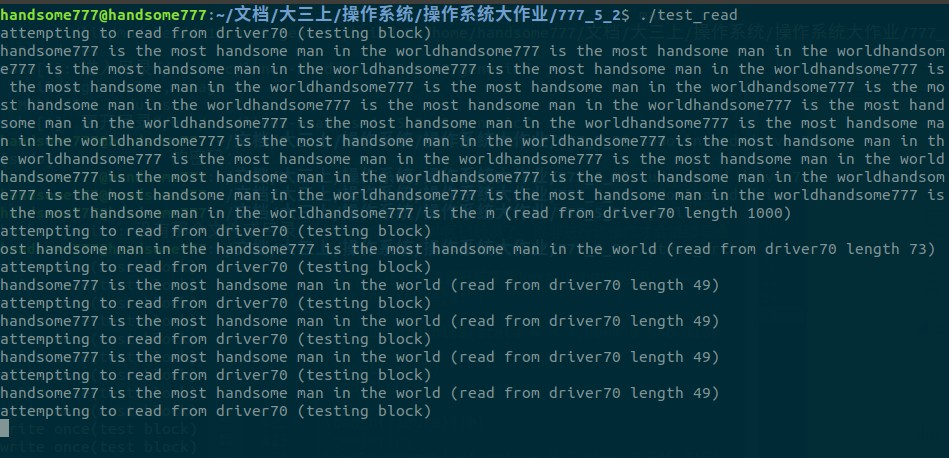
\includegraphics[scale = 0.7,bb=0 0 683 330]{5_9.jpg}
\label{img12}
\end{figure}
在kern.log中,结果如下:\par
\begin{figure}[!h]
\centering
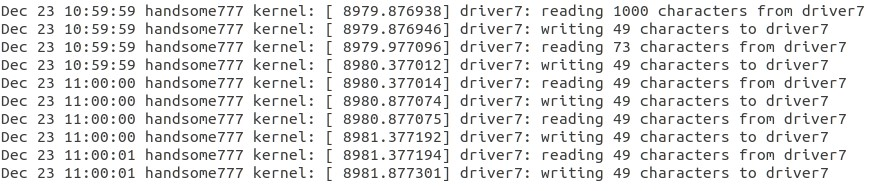
\includegraphics[scale = 0.7,bb=0 0 627 138]{5_10.jpg}
\label{img13}
\end{figure}
可以看到,第一次读取的是整个缓存区的内容,之后是写操作写一个,读操作就读一个。并且根据写入和读出的数据对比,发现是没有问题的,因此验证成功。

\subsection{代码运行顺序}
在终端依次输入如下命令:\par
make\par
gcc test$\_$write.c -o test$\_$write
gcc test$\_$read.c -o test$\_$read
sudo insmod driver7\par
./test$\_$write(在第一个终端)\par
./test$\_$read(在第二个终端)\par
ctrl+C ./test$\_$read\par
ctrl+C ./test$\_$write\par

\subsection{第三次实验总结}
本次试验用到了大量的linux中的调用,之前是完全没接触过的,因此查阅了很多参考资料,也阅读了一部分linux源码,反复理解并加以实践,才最终完成了本次实验,非常不容易。\par
本次试验最难的地方是在最开始的时候,并不清楚应该怎样写,应该如何设计框架,比较懵,后来一点一点摸索,查看了一些工具书,了解驱动开发的基本流程和细节。因为装的是linux双系统,并没有用虚拟机进行开发,所以在调试加载和卸载模块的时候,经常把电脑搞死机,因此必须得强制关机重启,这个代价比较大,所以这次实验花了比较久的时间。在进行读写操作调试的时候,一开始只运行write程序,陷入阻塞之后,已知ctrl+C没用,后来通过网上查资料才发现,我的操作是在用户空间中的,而阻塞是在内核中,因此杀死不掉程序。\par
通过这次实验,我了解了驱动开发的大概流程,通过对管道也有了更深的认识,更重要的是,对linux操作系统有了更深刻的认识,比如在内核进行操作的时候,可以通过用printk在kern.log中进行输出,根据输出进行结果调试。,收获很大!

\section{总结}
通过一学期的学习,并且加上三次实验,让我对操作系统有了更深刻的认识。第一次实验让我对进程进行了比较细致的了解,熟悉并掌握了多线程调试的方法,并且对互斥有了更深的认识。第二次试验是快速排序问题,因为第一次试验已经有了一定的基础,因此第二次实验上手特别快,思路比较清晰,第三次实验因为之前没有接触过相应的编程,因此花费了很多时间阅读资料书籍,虽然花了很多时间,但是非常有意义。三个实验都是在linux环境下进行开发的,因此我对Linux操作系统有一定的理解。\par
最后,感谢老师和助教对本课程的付出,感谢老师在课堂上的讲授,也感谢助教耐心负责地批改每一次小作业和三个实验!


\end{document}
